\documentclass{article}

% if you need to pass options to natbib, use, e.g.:
%     \PassOptionsToPackage{numbers, compress}{natbib}
% before loading neurips_2019

% ready for submission
% \usepackage{neurips_2019}

% to compile a preprint version, e.g., for submission to arXiv, add add the
% [preprint] option:
%     \usepackage[preprint]{neurips_2019}

\usepackage[final]{neurips_2019}
% to compile a camera-ready version, add the [final] option, e.g.:
% to avoid loading the natbib package, add option nonatbib:
%  \usepackage[nonatbib]{neurips_2019}

\usepackage[utf8]{inputenc} % allow utf-8 input
\usepackage[T1]{fontenc}    % use 8-bit T1 fonts
\usepackage{hyperref}       % hyperlinks
\usepackage{url}            % simple URL typesetting
\usepackage{booktabs}       % professional-quality tables
\usepackage{amsfonts}       % blackboard math symbols
\usepackage{nicefrac}       % compact symbols for 1/2, etc.
\usepackage{microtype}      % microtypography
\usepackage{graphicx}
\usepackage{float}
\documentclass[UTF8]{ctexart}
\usepackage{booktabs}
\usepackage{diagbox} 
\usepackage{multirow} 
\usepackage{makecell} 
\usepackage{array}
\usepackage{tabularx}
\usepackage{booktabs}%提供命令\toprule、\midrule、\bottomrule
\usepackage{multirow}%提供跨列命令\multicolumn{}{}{}


	
\title{(Re-)Imag(in)ing Price Trends:}

% The \author macro works with any number of authors. There are two commands
% used to separate the names and addresses of multiple authors: \And and \AND.
%
% Using \And between authors leaves it to LaTeX to determine where to break the
% lines. Using \AND forces a line break at that point. So, if LaTeX puts 3 of 4
% authors names on the first line, and the last on the second line, try using
% \AND instead of \And before the third author name.

\author{%
  Fu Yang \\
  21029346\\
  \texttt{yfubo@connect.ust.hk} \\
  \And
  Luo Yuqing \\
  20582315\\
  \texttt{yluobb@connect.ust.hk} \\
  \AND
  Wang Jinyuan \\
  21028990\\
  \texttt{jwangiy@connect.ust.hk} \\
  \And
  Wang Tong \\
  20905737\\
  \texttt{twangce@connect.hk} \\
}

\begin{document}

\maketitle

\begin{abstract}
This report discusses ...

\end{abstract}

\section{Introduction}

...

\section{Data}
\subsection{Data description}

In accordance with the article titled "(Re-) Imag(in)ing Price Trends,"^{[1]} our empirical analysis revolves around a panel prediction model for US stock returns using data from 1993 to 2019. The input data for this model depicts price and volume information over different time periods. Specifically, the data represents daily open, close, high, and low prices, as well as daily trading volume and moving average prices over the past 5, 20, and 60 days in the original paper. Our report focuses solely on the 20-day moving average. This decision is based on the notion that the long horizon entails a more complex network structure, which may impede computational efficiency. Conversely, the short horizon might oversimplify the analysis, potentially compromising the robustness of the conclusions drawn. Figure 1 displays a portion of the original data that was utilized to assess the accuracy of our predictions in subsequent analyses.

\begin{figure}[H]
	\centering
	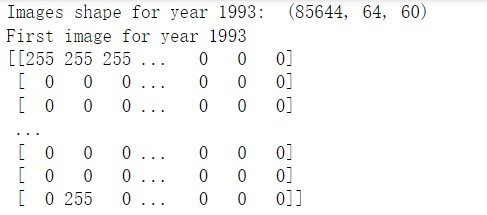
\includegraphics[width=0.8\textwidth]{Data/a1.png}
	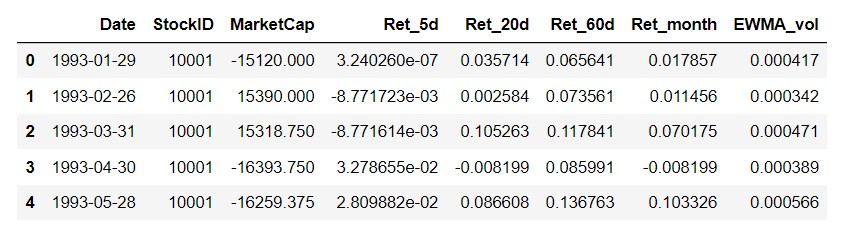
\includegraphics[width=0.8\textwidth]{Data/a2.png}
	\caption{Examples of Original Data}
\end{figure}

Below, we provide a segment of the comprehensive description that explains each label in detail.
\textbullet Date: The last day of the 20-day rolling window for the chart.
\textbullet StockID: CRSP PERMNO that identifies the stock.
\textbullet MarketCap: Market capitalization in dollar, recorded in thousands.
\textbullet Ret_{t}d: t=5,20,60, next t-day holding period return.
\textbullet Ret_month: Holding period return for the next month, from the current monthend to the next month end.
\textbullet EWMA_vol: Exponentially weighted volatility (square of daily returns) with alpha as 0.05. One day delay is included.

To facilitate analysis, the original dataset was partitioned into three distinct categories based on the returns observed. Within this categorization, a value of 0 was assigned to instances characterized by non-positive returns. Conversely, instances exhibiting positive returns were assigned a value of 1.

\subsection{Data exploration}
The data processing stage involves further transformations and modifications to the prepared dataset. 

The primary objective of transforming the original one-dimensional time series of stock data into two-dimensional images is to improve the prediction accuracy of the model. This is achieved for several reasons. Firstly, the use of images allows for more effective processing by convolutional neural networks (CNNs), which excel at image analysis. This enables the model to extract meaningful features and patterns from the data. Secondly, the conversion of time series into images enhances the model's ability to predict stock data by providing a visual representation that captures important relationships and trends. And then by combining price and trading volume data within the same image, the model gains a more comprehensive understanding of the data, leading to improved prediction effectiveness. Ultimately, the goal is to predict stock price trends, making this image encoding approach particularly suitable for technical trading analysis.

The constructed images in the original paper have unique characteristics that set them apart. Daily data points are consolidated into 20-day intervals, and the height of all images is standardized by scaling the vertical axis. This standardized representation enables easy comparison and analysis across different stocks. 

Instead of utilizing a candlestick chart, we opted for "OHLC" (Open-High-Low-Close) bars in the image representation. OHLC bars convey the same information while using fewer pixels, optimizing visual space.

The images, now at a resolution of 64×60 pixels, have been augmented with additional features. Moving average lines (MA) and volume bars (VB) are incorporated to provide a more comprehensive representation of price trends and trading activity. This augmentation enhances the visual information available to the model.

To optimize data storage and processing efficiency, all "Image" data has been transformed into binary form. The pixel values, originally ranging from 0 to 255, are standardized to a binary range of 0 or 1. This reduction in data size from a continuous scale to a binary representation minimizes memory requirements and enables faster computations. 

\begin{figure}[ht]
	\centering
	\begin{minipage}[b]{0.49\linewidth}
		\centering
		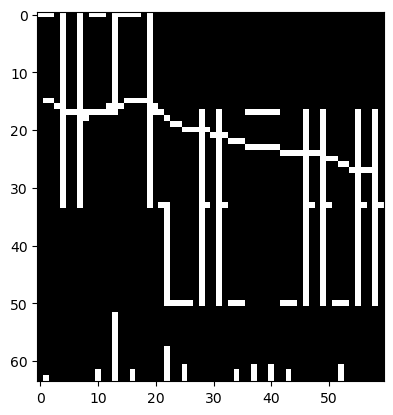
\includegraphics[width=0.8\linewidth]{Data/a3.1.png} 
	\end{minipage}
	\hfill
	\begin{minipage}[b]{0.49\linewidth}
		\centering
		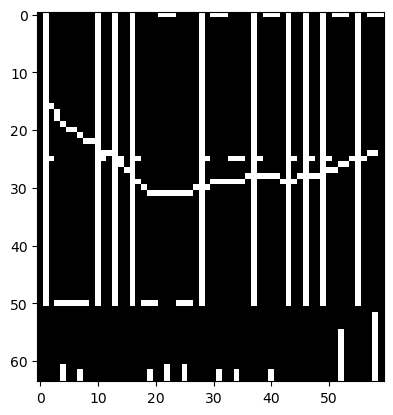
\includegraphics[width=0.8\linewidth]{Data/a3.2.png} 
	\end{minipage}
	\caption{Examples of Final Image}
\end{figure}

After extensive efforts, we successfully generated an image(eg. Figure 2 ) that incorporates the stock price, moving average lines, and volume bars. These features were carefully designed to be compatible with the CNN model, ensuring optimal utilization of the image representation for analysis and prediction purposes.

Finally, To ensure the robustness of the model, the dataset was divided into three subsets: training, validation, and testing samples. Following the approach outlined in the original paper, the first seven-year sample from 1993 to 1999 was utilized for training and validation purposes. Specifically, 70\% of the sample was randomly selected for training the model, while the remaining 30\% was allocated for model validation. This division strategy allows for rigorous evaluation and validation of the model's performance.

\section{Architecture Design}
A Convolutional Neural Network (CNN) is a deep learning algorithm designed for image analysis and object recognition. It takes an input image, identifies important objects within it, and distinguishes one object from another. By stacking together a sequence of operations, a CNN transforms a raw image into a set of predictive features and makes a final prediction. 

One of the primary reasons we choose the Convolutional Neural Network (CNN) model is due to its numerous advantages in processing image data.

First and foremost, CNNs offer a significant advantage in terms of parameter efficiency. Unlike traditional feed-forward neural networks, CNNs impose cross-parameter restrictions that dramatically reduce parameterization. This reduction in parameters makes CNNs more tractable to train and optimize, particularly when working with large-scale image datasets. By requiring fewer parameters, CNNs can effectively capture and represent the complex features present in images while mitigating the computational and data requirements associated with generic unconstrained neural networks.

Another key advantage of CNNs is their ability to handle variations in object position, scale, and orientation. Traditional neural networks are inherently sensitive to such changes, which hampers their effectiveness in recognizing and analyzing objects in different contexts. In contrast, CNNs excel at addressing this challenge. Through the use of convolutional layers, pooling layers, and spatial hierarchies, CNNs embed tools within their architecture that make the model resilient to deformation and re-positioning of important objects in an image. This resilience allows CNNs to capture local patterns and features in an image, irrespective of their specific location or arrangement. Consequently, CNNs are better equipped to handle real-world scenarios where objects may appear in different positions or undergo transformations.

Furthermore, CNNs have been proven to be highly effective in image-related tasks. Their success in tasks such as image classification, object detection, and image segmentation has made them the go-to model for image analysis and processing. CNNs' ability to extract and learn hierarchical representations from raw image data enables them to capture intricate details and discriminative features, leading to superior performance in various image-based applications. 

The key operations in a CNN's building block are convolution, activation, and pooling, 

\subsection{Convolution}
Convolution is a process that is similar to kernel smoothing. It involves scanning an image both horizontally and vertically. For each element in the image matrix, a summary of the surrounding area is computed.

In convolution, a set of filters is used. A filter is a small matrix of weights.In our project, 64 filters were employed, each with a kernel size of 5x3. We use 3 blocks for 20-day images. 

To safeguard the data from loss, a padding function is added. Padding involves adding extra pixels to each side of the image to prevent the feature map from becoming too small. The number of pixels added is determined by the size of the filter and the stride. 

So here we applies a 2D convolution over an input signal composed of several input planes with ‘CONV2D’,

\textbullet\emph{ input:(N, C^{in}, H^{in}, W^{in}) or (C^{in}, H^{in}, W^{in})}
\textbullet\emph{output:(N,C^{out}, H^{out}, W^{out}) or (C^{out}, H^{out}, W^{out})}, where

\emph{H^{out} = \left[\frac{H^{in} + 2 * padding[0] - dilation[0] * (kernel_size[0]-1)-1}{stride[0]} + 1]\right}

\emph{W^{out} = \left[\frac{W^{in} + 2 * padding[1] - dilation[1] * (kernel_size[1]-1)-1}{stride[1]} + 1]\right}

For example, on the first layer the first operation is a Conv2d layer with an input of 1 channel, outputting 64 channels. It uses a kernel size of (5, 3), a stride of (3, 1), padding of (12, 1), and dilation of (2, 1).  

Furthermore, batch normalization is incorporated into the design of the Convolutional Neural Network (CNN) model to counteract overfitting. Batch normalization is a layer that enables each layer of the network to learn more independently. It normalizes the output of the previous layers and effectively prevents overfitting through regularization. It is particularly effective in CNNs.

Here we applies Batch Normalization over a mini-batch of 2D inputs with additional channel dimension with ‘BATCHNORM2D’, and in the shape,

\emph{y = \frac{x-E[x]}{\sqrt{Var[x]+\epsilon}} * \gamma + \beta }

\textbullet input:\emph{(N, C, H, W)}
\textbullet output:\emph{(N, C, H, W)} (same shape as input)

The second operation of batch normalization is a BatchNorm2d layer with 64 channels. 

\subsection{Activation}
In a Convolutional Neural Network (CNN), the activation operation is a crucial step that follows the convolutional operation. It introduces non-linearity into the network, enabling it to learn complex patterns and make accurate predictions. The activation operation applies a non-linear transformation element-wise to the output of a convolutional filter.

The choice of the activation function plays a significant role in the effectiveness of the CNN. In the case you mentioned, the "leaky ReLU" activation function is used. The leaky ReLU addresses the limitation of the standard ReLU activation function, known as the "dying ReLU" problem. The dying ReLU problem occurs when some neurons get stuck in a negative state and cease to contribute to the learning process. By using the leaky ReLU activation function, the CNN can learn more robust and expressive representations of the input data. It avoids the complete suppression of negative values, allowing some information to flow through and preventing neurons from becoming inactive.

For example, On layer1 the second operation is a BatchNorm2d layer with 64 channels. And the third operation is a LeakyReLU activation function with a negative slope of 0.01.

\subsection{Pooling}

Pooling is an operation in a convolutional neural network (CNN) that serves two main purposes. Firstly, it reduces the dimensionality of the data by removing redundant information. Secondly, it acts as a de-noising tool, enhancing the network's robustness by focusing on the most important features and suppressing noise. Pooling, particularly max-pooling, selects the maximum value within each region, reducing the spatial dimensions while retaining key features. This helps control computational complexity, improve memory efficiency, and enhance the network's ability to generalize well to new data.

Here we applies a 2D max pooling over an input signal composed of several input planes with ’MAXPOOL2D’, and in this shape

\textbullet\emph{ input:(N, C, H^{in}, W^{in}) or (C, H^{in}, W^{in})}
\textbullet\emph{output:(N,C, H^{out}, W^{out}) or (C, H^{out}, W^{out})}, where

\emph{H^{out} = \left[\frac{H^{in} + 2 * padding[0] - dilation[0] * (kernel_size[0]-1)-1}{stride[0]} + 1]\right}

\emph{W^{out} = \left[\frac{W^{in} + 2 * padding[1] - dilation[1] * (kernel_size[1]-1)-1}{stride[1]} + 1]\right}

For example, On layer1 the fourth operation is a MaxPool2d layer with a kernel size of (2, 1), a stride of (3, 1), padding of 0, and dilation of (2, 1).

The final architecture of the baseline model is as the figure shows below.

\begin{figure}[H]
	\centering
	\includegraphics[width=0.8\textwidth]{Diagram of CNN Models.png}
	\caption{ Diagram of CNN Models }
\end{figure}

In addition, Our research suggests embedding time series data as images before conducting predictive analysis. This approach offers several advantages over directly modeling the time series. By representing the data as images, convolutional filters can capture non-linear spatial associations among different price curves, enabling the detection of complex patterns that may be missed by traditional time series modeling. Additionally, the image representation combines information on price movements, trends, volatility, and trading volume into a single representation, eliminating the need for manual feature engineering and non-linear transformations. Ingesting data as images allows the model to isolate data relationships that are challenging to detect using conventional time series methods. Similar to how humans find it easier to identify patterns graphically, a statistical pattern recognition algorithm can benefit from visualizing the data matrix as a single image.

\section{Working Flow}

\subsection{Data split}
Our workflow follows a standard procedure, starting with training the model, followed by model tuning, and finally making predictions. We divide the data samples into three sets: training, validation, and testing. Following the original paper, we also used a seven-year sample from 1993 to 1999 for training and validation. Within this sample, 70\% of the data was randomly selected for training the model, while the remaining 30\% was used for validation. The remaining twenty years of data were reserved as an out-of-sample test dataset.

\subsection{Regularization procedures}
To build a baseline CNN model for 20-day images, we followed the paper and applied several regularization procedures to combat overfitting and improve computational efficiency, including the Xavier initialization, dropout, batch normalization and early-stopping.

\textbullet \textbf{Xavier initializer}
We utilize the Xavier initializer, as proposed by Glorot and Bengio(2010)^{[2]}, to initialize the weights in each layer of our model. It initializes the weights based on the dimensions of the input and output, equalizing the variances of the two dimensions. This helps avoid the issues of vanishing or exploding gradients and promotes convergence of the network. By applying the Xavier initializer, we aim to improve the training efficiency and performance of our model.

\textbullet \textbf{Batch normalization}
We incorporate batch normalization in our CNN model design to address the issue of covariate shift and prevent overfitting. The batch normalization layer, as proposed by Ioffe and Szegedy(2015)^{[3]}, is placed between the convolutional layer and the non-linear activation function within each building block. Batch normalization is a technique that normalizes the output of the previous layers in the network and allows each layer to learn more independently. It is particularly effective in CNN models. By normalizing the inputs of each mini-batch, batch normalization helps stabilize the network with respect to variations in the input data. This leads to accelerated convergence during training and provides some regularization effects, reducing the risk of overfitting.

\textbullet \textbf{Dropout}
We incorporate the dropout regularization technique in our model to mitigate overfitting. During training, we apply a dropout rate of 50\% to the fully connected layer, as recommended by Srivastava et al. (2014)^{[4]}. This means that in each training iteration, there is a 50\% chance of dropping out each neuron in the fully connected layer. By randomly deactivating neurons, the network is encouraged to rely on other neurons, promoting robustness and improving generalization. It is important to note that we do not apply dropout in the convolutional blocks since their relatively low parameterization already helps avoid the need for dropout in those layers. By incorporating dropout, we introduce randomness into the network, preventing it from relying too heavily on specific features or neurons. This regularization technique improves the stability and robustness of our model, allowing it to perform better on unseen data and reducing the risk of overfitting.

\textbullet \textbf{Early stopping}
We utilize early stopping as a strategy to prevent overfitting in our training process. Early stopping involves monitoring the performance of the model on a separate validation set during training. If the performance on the validation set fails to improve for two consecutive epochs, we halt the training process. By implementing early stopping, we ensure that the model is not trained for an excessive number of epochs, which can lead to overfitting. When the model's performance on the validation set plateaus or starts to decline, it indicates that further training may not improve the model's generalization capability. Stopping the training process at this point helps us avoid overfitting and enhances the model's ability to generalize to unseen data.

\subsection{Loss and evaluation}
\textbullet \textbf{Cross Entropy Loss}
In our prediction analysis, we approach it as a classification problem. We define the label for an image as y = 1 if the subsequent return is positive, indicating a positive outcome, and y = 0 otherwise, representing a negative outcome.

To measure the performance of our model, we utilize the Cross Entropy Loss as our loss function. Cross Entropy Loss is commonly used in classification tasks and is well-suited for evaluating the performance of models that predict probabilities across multiple classes. It quantifies the difference between the predicted probabilities and the true labels, providing a measure of how well the model is able to classify the input data.

By employing Cross Entropy Loss as our loss function, we aim to optimize our model's parameters to minimize the discrepancy between predicted probabilities and the true labels. This enables our model to learn and improve its classification performance, ultimately enhancing its ability to accurately predict the subsequent returns.

\emph{L_{CE}(y, \hat{y}) = -ylog(\hat{y}) - (1-y)log(1-\hat{y})
	
Where the softmax output, \hat{y} , from the final step of our CNN model as the prediction, and y represents the ground truth label. The loss function we employ is designed to quantify the discrepancy between the predicted probabilities and the true labels. If the predicted probability exactly matches the ground truth label, the loss function is zero. Otherwise, the loss function returns a positive value, indicating the degree of disagreement between the prediction and the true label.

We optimize the loss function using stochastic gradient descent (SGD) with the Adam algorithm. The initial learning rate is set to 1×10^(-5), and we use a batch size of 128 to handle memory constraints. The training process involves 100 epochs, and we employ early stopping if the loss function does not improve on the validation set for two consecutive epochs.

\begin{figure}[H]
	\centering
	\includegraphics[width=0.8\textwidth]{CNN_loss.png}
	\caption{CNN classification loss}
\end{figure}

Figure shows the training loss of our CNN classification model over time. The y-axis represents the loss function, which measures the difference between the predicted output and actual label. The x-axis indicates the number of training iterations.

The loss function decreasing over time signifies the learning and enhancement of our model's classification performance. The plot includes a moving average of the loss function, which offers a smoother representation and highlights the overall trend. This moving average is computed by averaging the loss function values over a sliding window of 20 training iterations. Figure 3 presents a visual depiction of the training and evaluation loss functions for our CNN classification model. The x-axis denotes the number of training epochs, while the y-axis represents the value of the loss function.

\begin{figure}[H]
	\centering
	\includegraphics[width=0.8\textwidth]{ CNN classification training and evaluation loss.png}
	\caption{ CNN classification training and evaluation loss}
\end{figure}

The subplot on the left depicts the training loss function, which quantifies the disparity between the predicted output and the actual label on the training data. A decreasing trend in the training loss function indicates that our model is learning and enhancing its classification performance on the training data. The vertical red line denotes the checkpoint where early stopping was employed to prevent overfitting, highlighting the effectiveness of this strategy.

The subplot on the right illustrates the evaluation loss function on the validation dataset. This loss function measures the difference between the predicted output and the actual label on the validation data, providing an assessment of the model's generalization ability. A decreasing trend in the evaluation loss function suggests that our model is consistently learning and improving its classification performance on new data. The vertical red line also signifies the checkpoint where early stopping was triggered during training, demonstrating that the model exhibits good generalization capabilities.

	
\textbullet \textbf{Accuracy}
We measure the classification accuracy using the Accuracy metric. This metric represents the ratio of correct determinations to the total number of determinations.

To calculate the accuracy, we consider true positive (TP) and true negative (TN) predictions. A TP occurs when the predicted probability is greater than 50\% and corresponds to a positive realized return. Similarly, a TN occurs when the predicted probability is less than 50\% and coincides with a negative return. On the other hand, false positives (FP) and false negatives (FN) represent incorrect predictions. FP indicates a positive prediction that does not align with the negative realized return, while FN indicates a negative prediction that does not coincide with the positive realized return.

The accuracy is calculated by summing the number of TP and TN predictions and dividing it by the total number of predictions, which includes TP, TN, FP, and FN. This formula provides a measure of how well our model performs in classifying the outcomes.

\emph{Accuracy = \frac{TP + TN}{TP + TN + FP + FN}}

we visualized the classification results of the model on a sample of test images, which demonstrated its ability to accurately predict the direction of returns, as illustrated in Figure .

\begin{figure}[H]
	\centering
	\includegraphics[width=0.8\textwidth]{CNN classification visualized results.png}
	\caption{CNN classification visualized results}
\end{figure}


\textbullet \textbf{Classification Performance}
Table below illustrates the classification performances of our model after employing various regularization techniques. These procedures contribute to the improved classification performance of our model. 


\begin{table}[H]
	\caption{\textbf{Performance Comparison}}
	\centering
	\begin{tabular}{ccccc}
		\toprule
		&&\multicolumn{2}{c}{\textbf{\underline{Baseline(Paper)}}}&\multicolumn{2}{c}{\textbf{\underline{Baseline(Replication)}}} \\
		\midrule%第二道横线 
		&& Test  & Val  & Test  & Val   \\ 
		&Accuracy  & 0.533  & 0.542  & 0.513  & 0.499 \\
		&Loss  & 0.690  & 0.687  & 0.714  & 0.704 \\
		\bottomrule%第四道横线
	\end{tabular}
\end{table}
	

The analysis reveals that the classification model demonstrates convergence as the number of iterations increases. The relationship between cross-entropy loss and accuracy over epochs indicates stable performance on the train and validation datasets, with a loss value of approximately 0.7 and an accuracy range of 0.50-0.54. The model's performance on the test dataset closely matches the results reported in the paper, with a loss value of 0.714 and an accuracy of 0.513. Overall, the model exhibits satisfactory convergence and generalization abilities.

\section{Extension}

\subsection{Ablation Studies}
To test the robustness of the CNN model, we follow the methodology outlined in Appendix B of the original paper and conduct a similar sensitivity analysis. We introduce various modifications to both the model architecture(e.g. number of convolution layers) and estimation(e.g. dropout rate or batch normalization schemes). The performance of the models are evaluated by loss, accuracy from test and validation process and the Pearsonr and Spearmanr correlation. Detailed variations of the model and their performance are shown in the table below.

Table

The ablation studies reveal that CNN model’s performance is considerably robust and exhibits low sensitivity to alterations in modeling choices. 

\subsection{Interpretability}
CNN models are highly flexible and capable of automatically learning complex predictive patterns from data, eliminating the need for manual feature engineering. In this project, interpreting the model's decisions and understanding its reasoning process are crucial for gaining insights into the factors that influence stock price movements. However, interpreting the patterns discovered by CNN models can be challenging due to their lack of decomposability into individually intuitive components. [2] In this context, visualization explanation techniques can be helpful. Therefore, we apply the Gradient-weighted Class Activation Mapping (Grad-CAM) method, as suggested by the original paper, to facilitate the interpretation process.

Grad-CAM identifies the most important regions within the input image that contributes to the model’s prediction. Compared with some other CNN visualization techniques, Grad-CAM is highly class-discriminative, and it uses the gradient information flowing back into the last convolutional layer of the CNN to assign importance values to each neuron for a particular decision of interest.[3] These values are then used to create a weighted combination of the feature maps, resulting in a heat map that highlights the regions most relevant to the predicted class.

The output of Grad-CAM is a heatmap that overlays the input image, indicating the regions that the model considers important for its decision. Higher intensity regions in the heatmap correspond to areas that strongly influence the prediction, while lower intensity regions are deemed less influential.

We randomly select 10 images each for predicted movements “up” and “down” and the heap maps generated are shown below.

\begin{figure}[H]
	\centering
	\includegraphics[width=0.8\textwidth]{Figure for Up.png}
	\caption{Figure for Up}
\end{figure}

\begin{figure}[H]
	\centering
	\includegraphics[width=0.8\textwidth]{Figure for down.png}
	\caption{Figure for down}
\end{figure}

\subsection{Regression}
We expand our scope beyond binary classification and attempt to predict numerical values. The input remains to be the 20-day horizon images, representing historical stock movements and predictions are modified to be the next 5-day and 20-day holding period returns. To accommodate numerical predictions, we retain the overall structure of the CNN model while making two key changes: adjusting the loss function to Mean Squared Error (MSE) and changing the activation function in the output layer to linear instead of softmax. The figures below depict the MSE and early stopping checkpoint for both models.

Figure

The unsatisfactory performance of both regression models, as indicated by negative R-squared values, could be attributed to multiple factors. One possible reason is insufficient input data, which can limit the model's ability to learn meaningful patterns and relationships. Additionally, the pooling and downsampling operations of CNN model may result in a loss of fine-grained information that is important for precise numerical predictions in regression tasks.

\section{Conclusion}

In this project, we successfully replicate the research paper by closely adhering to the original work's guidelines for data preparation, model design, workflow, and performance evaluation and our replication yields similar results. Moreover, we conduct ablation studies to assess the model's robustness, utilize Grad-CAM to interpret the CNN and identify crucial patterns for prediction, and extend our exploration to regression analysis. 


\section*{References}

\medskip

\small


[1] Jiang J, Kelly B T, Xiu D. (Re-) Imag (in) ing price trends[J]. Chicago Booth Research Paper, 2020 (21-01).
[2] Glorot, Xavier, and Yoshua Bengio, 2010, Understanding the difficulty of training deep feedforward neural networks, in Proceedings of the thirteenth international conference on artificial intelligence and statistics, 249–256.
[3] Ioffe, Sergey, and Christian Szegedy, 2015, Batch normalization: Accelerating deep network training by reducing internal covariate shift, arXiv preprint arXiv:1502.03167 . 
[4] Z.C.Lipton.TheMythosofModelInterpretability.ArXive-prints, June 2016.
[5] Selvaraju, R. R., Cogswell, M., Das, A., Vedantam, R., Parikh, D., & Batra, D. (2017). Grad-CAM: Visual Explanations from Deep Networks via Gradient-based Localization. In Proceedings of the IEEE International Conference on Computer Vision (ICCV), 618–626.



\section*{Group contribution}
Wang Jinyuan: Coding
Fu Yang: Coding Support and Report writing part of data, Architecture Design and Working Flow, Latex formatting
Luo Yuqing: Coding Support and Report writing part of Abstract, Introduction and Extension
Wang Tong: Coding Support

All members participate actively and equally contribute to this project.

\section*{Github link}
https://github.com/dboywjy/Home\_Credit\_Default\_Risk\_LFWW/tree/hcdr\_wjy2

\end{document}
